\documentclass{article}

\usepackage{graphicx}
\usepackage{tikz}
\usepackage{tikzsymbols}
\usetikzlibrary{calc,patterns,shapes.geometric}
\pagestyle{empty}
\usepackage[margin=0pt]{geometry}
\geometry{papersize={14in,12in}}

\def\centerarc[#1](#2)(#3:#4:#5){\draw[#1] ($(#2)+({#5*cos(#3)},{#5*sin(#3)})$) arc (#3:#4:#5);}

\begin{document}
	\begin{figure}
		\centering
		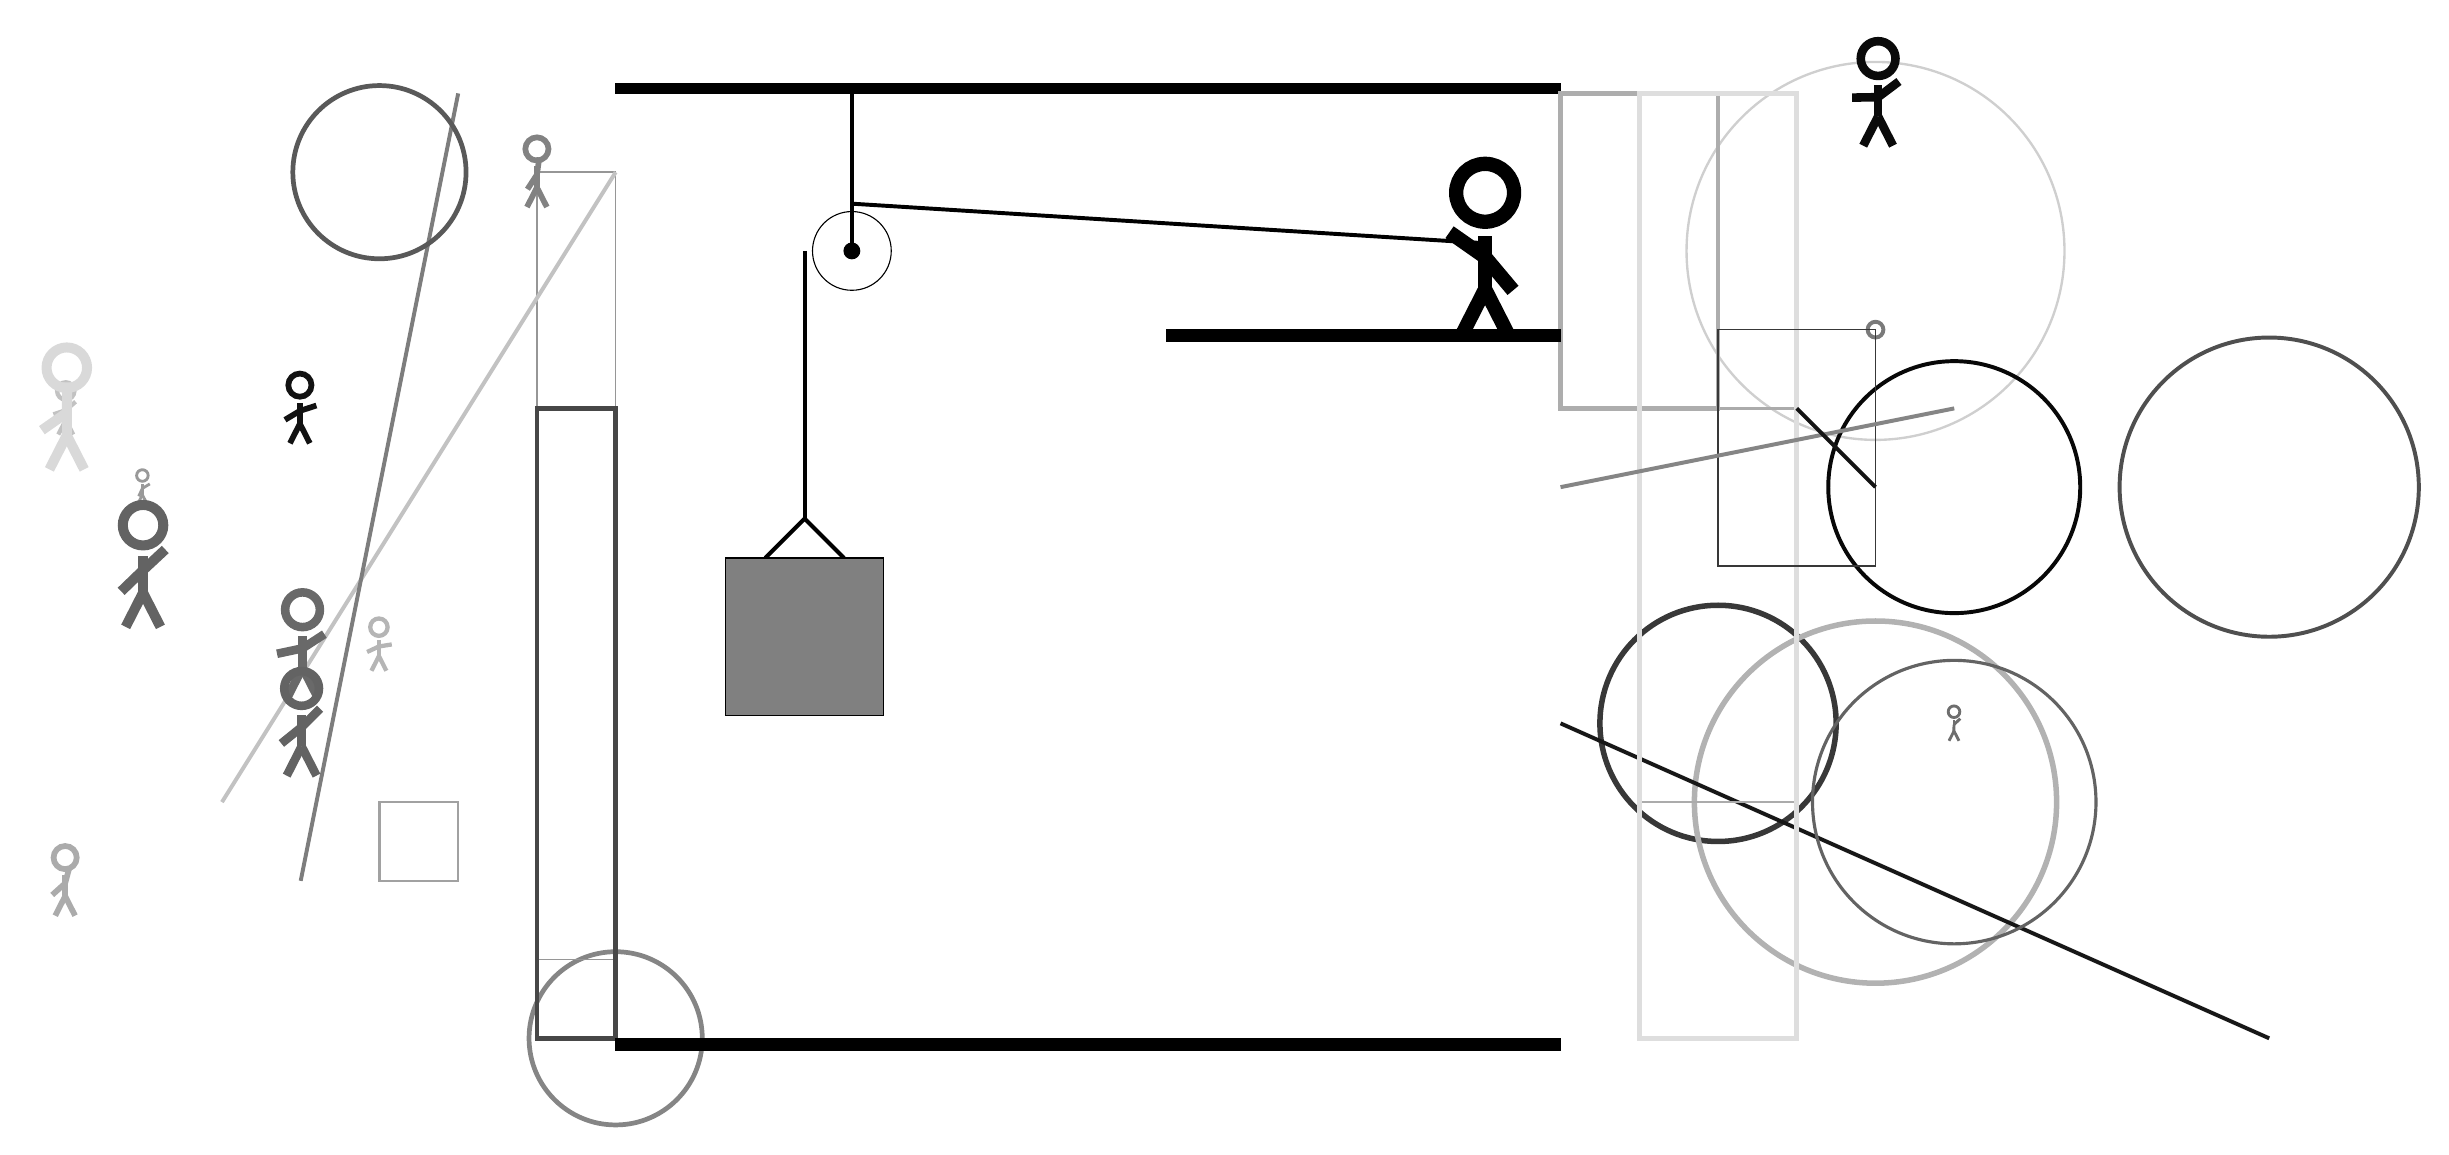
\begin{tikzpicture}
			%%%%% START %%%%%
			
			\draw[fill=black] (-2, 9) rectangle (10, 9.125);
			
			\draw (1, 7) circle (0.5);
			\draw[fill=black] (1, 7) circle (0.1);
			\draw[line width=0.5mm] (1, 9) -- (1, 7);
			
			\node[line width=0.7mm, color=black!57] at (15, 1) {\Strichmaxerl[2][88][44]};
			
			\draw [line width=0.7mm, color=black!78](12, 1) circle (1.5);
			\draw [line width=0.6mm, color=black!48](-2, -3) circle (1.1);
			\draw [line width=0.7mm, color=black!30](14, 0) circle (2.3);
			\draw[line width=0.2mm, color=black!41] (-3, -2) rectangle (-2, 8);
			\draw [line width=0.3mm, color=black!19](14, 7) circle (2.4);
			
			\draw[line width=0.5mm, color=black!91](10, 1) -- (19, -3);
			\node[line width=0.2mm, color=black!96] at (14, 9) {\Strichmaxerl[6][1][37]};
			\draw[line width=0.3mm, color=black!33] (11, 5) rectangle (13, 0);
			\draw [line width=0.5mm, color=black!97](15, 4) circle (1.6);
			
			\node[line width=0.6mm, color=black!24] at (-9, 5) {\Strichmaxerl[3][18][41]};
			\draw[line width=0.6mm, color=black!32] (10, 9) rectangle (12, 5);
			\node[line width=0.2mm, color=black!29] at (-5, 2) {\Strichmaxerl[3][25][9]};
			\draw[line width=0.5mm, color=black!24](-7, 0) -- (-2, 8);
			\draw[line width=0.5mm, color=black!51](-4, 9) -- (-6, -1);
			\draw [line width=0.4mm, color=black!61](15, 0) circle (1.8);
			\draw[line width=0.6mm, color=black!72] (-3, -3) rectangle (-2, 5);
			\draw[line width=0.6mm, color=black!13] (11, 9) rectangle (13, -3);
			\node[line width=0.6mm, color=black!49] at (-3, 8) {\Strichmaxerl[4][57][82]};
			\draw[line width=0.3mm, color=black!37] (-4, -1) rectangle (-5, 0);
			\node[line width=0.5mm, color=black!59] at (-6, 2) {\Strichmaxerl[6][12][33]};
			
			\node[line width=0.5mm, color=black!15] at (-9, 5) {\Strichmaxerl[7][35][89]};
			\draw [line width=0.5mm, color=black!52](14, 6) circle (0.1);
			\draw[line width=0.2mm, color=black!78] (12, 6) rectangle (14, 3);
			\draw [line width=0.6mm, color=black!65](-5, 8) circle (1.1);
			
			\node[line width=0.7mm, color=black!40] at (-8, 4) {\Strichmaxerl[2][65][31]};
			\node[line width=0.7mm, color=black!61] at (-6, 1) {\Strichmaxerl[6][39][45]};
			\draw[line width=0.5mm, color=black!48](10, 4) -- (15, 5);
			
			\draw [line width=0.5mm, color=black!69](19, 4) circle (1.9);
			
			\draw[line width=0.5mm, color=black!92](13, 5) -- (14, 4);
			\node[line width=0.4mm, color=black!33] at (-9, -1) {\Strichmaxerl[4][42][75]};
			
			\node[line width=0.3mm, color=black!93] at (-6, 5) {\Strichmaxerl[4][31][18]};
			\node[line width=0.3mm, color=black!61] at (-8, 3) {\Strichmaxerl[7][44][43]};
			
			\draw[line width=0.5mm](-0.1, 3.1) --  (0.4, 3.6) -- (0.9, 3.1);
			\draw[fill=black!50] (-0.6, 3.1) rectangle (1.4, 1.1);
			
			\draw[line width=0.5mm](0.4, 7) -- (0.4, 3.6);
			\centerarc[line width=0.5mm](1, 7)(90:180:0.6)
			\draw[line width=0.5mm](1, 7.6) -- (9, 7.1);
			
			\node at (9, 7) {\Strichmaxerl[10][-35][-50]};
			\draw[fill=black] (5, 6) rectangle (10, 5.85);
			
			\draw[fill=black] (-2, -3) rectangle (10, -3.15);
			
			%%%%% END %%%%%
		\end{tikzpicture}
	\end{figure}	
\end{document}